% vim: set spell : spelllang=en_gb
\title{\bf Dynamic priority broadcasting channels:\\
	a multi-objective planning problem}
\author{Chiel Kooijman - 5743028\\University of Amsterdam}
\documentclass{article}
\usepackage{graphicx,amsmath}
\usepackage[round]{natbib}
\usepackage{multicol}
\usepackage{caption}
\usepackage{subcaption}
\usepackage{geometry}
\def\keywords{\vspace{.5em}
	{\textbf{Keywords}:\,\relax
}}
\def\endkeywords{\par}
\newenvironment{tablehere}
{\def\@captype{table}}
{}

\newenvironment{figurehere}
{\def\@captype{figure}}
{}

\date{}
\setlength{\textwidth}{6.5in}
\setlength{\oddsidemargin}{0in}
\setlength{\evensidemargin}{0in}
\thispagestyle{empty}
\begin{document}
	\maketitle
	\begin{keywords}
		Dynamic Programming, MDP, Markov Decision Process, Multiobjective,
		Planning, Broadcasting Channel, Dynamic Priority
	\end{keywords}


	\begin{multicols}{2}

	\section{Introduction}
	\label{sec:introduction}
	In this research we extend the broadcasting channel problem as defined by
	\citet{ooi1996decentralized}, in order to account for situations in which
	multiple objectives are important, such as workload distribution in a data
	environment, distribution of traffic, or prioritisation of more important
	messages, in addition to throughput.
	In section \ref{sec:problem_definition} we redefine the problem to account
	for these considerations. Section \ref{sec:approach} covers the methods used
	to meet these requirements.
	% section introduction (end)

	\section{Problem definition}
	\label{sec:problem_definition}
	Multiple agents broadcast messages over a single channel, but only one
	message can be sent at any time, otherwise conflicts will arise and no
	message will come through. After a message is sent, the agents will know
	whether a message was sent, a conflict has arisen, or no message was sent.
	Agents have a single buffer that may contain a message. An example of a
	two-agent setup is shown in figure \ref{fig:agents_ee}.

	\begin{figurehere}
		\centering
		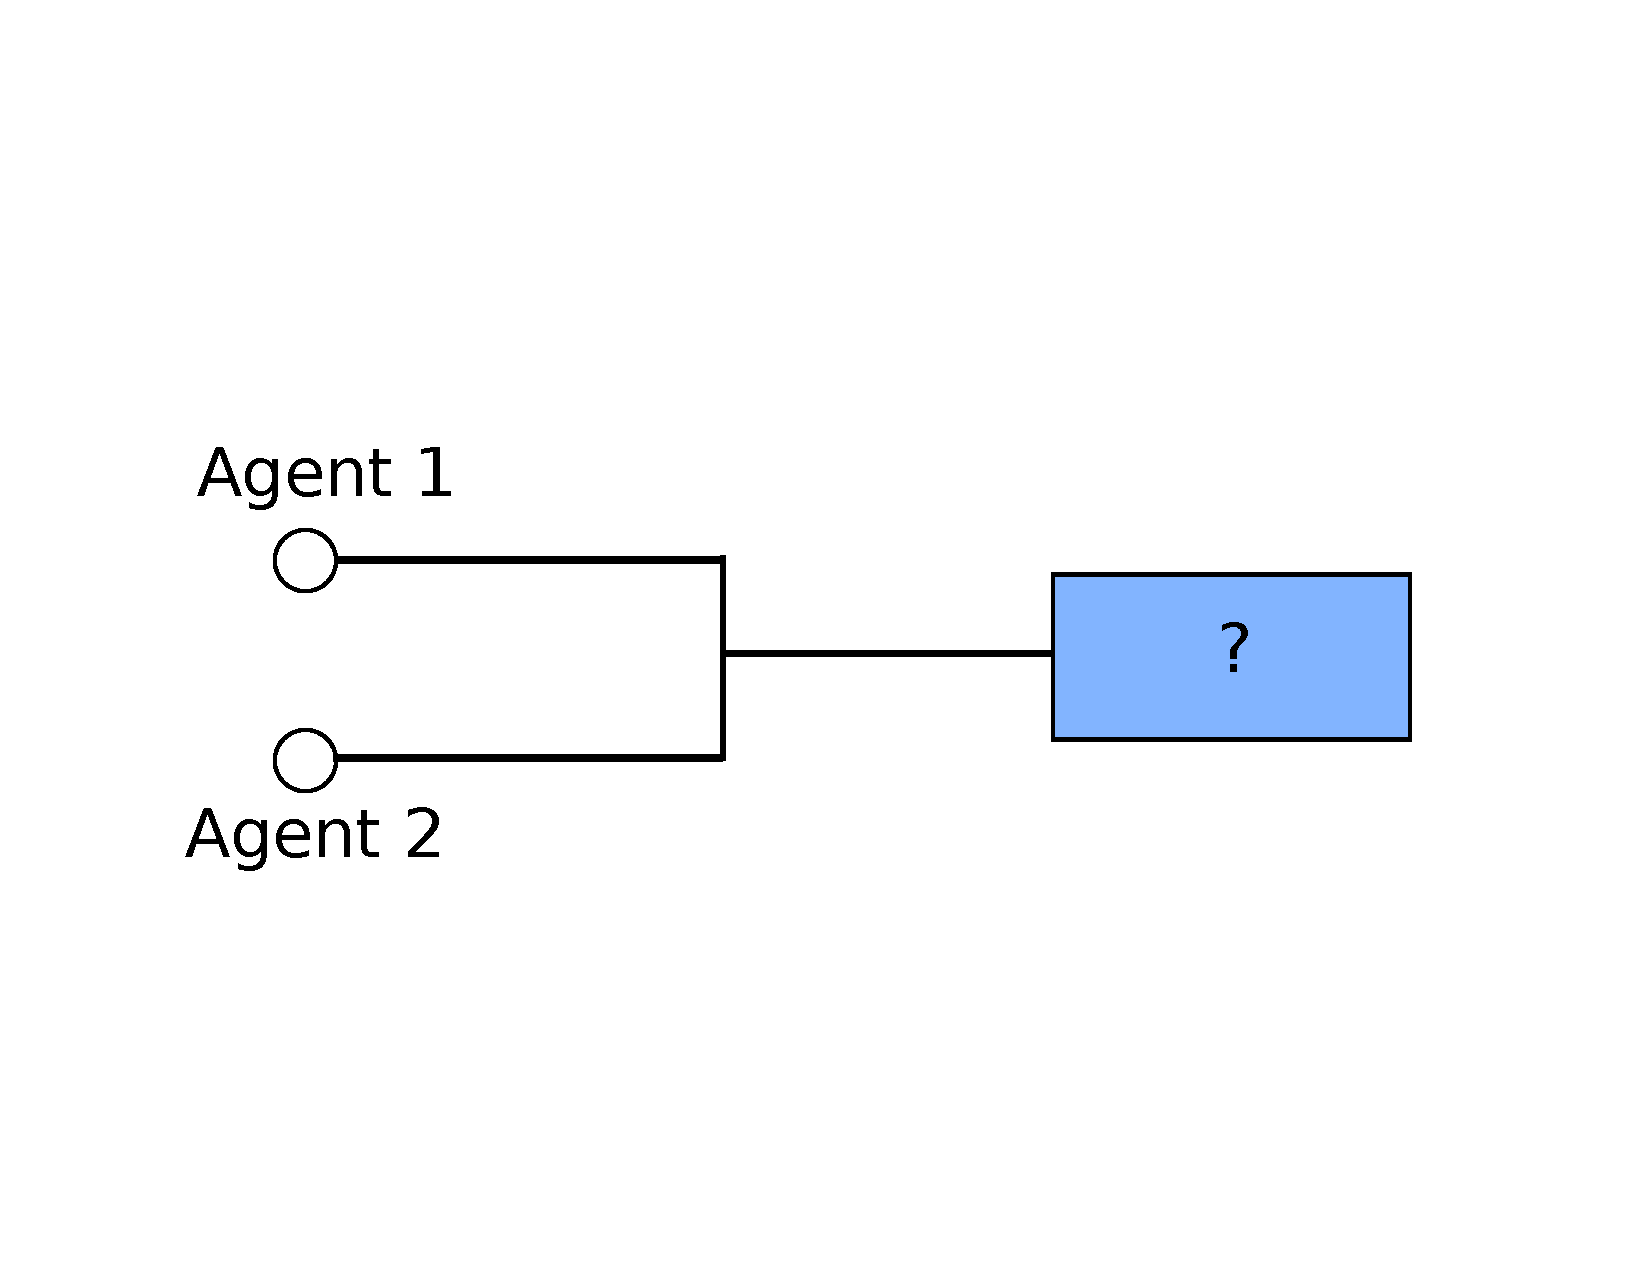
\includegraphics[scale=0.3]{images/agents_ee}
		\captionof{figure}{A setup with two agents}
	   \label{fig:agents_ee}
	\end{figurehere}

	At any concrete time-step an agent $i$ with an empty buffer may get a new
	message with probability $p_i(s' |s, \vec{a})$ in a fully observable Markov
	decision process (MDP), and $p_i(s' \vec{o}|s, \vec{a})$ in a partially
	observable Markov decision process (POMDP) \citep{hansen2004dynamic}.

	The problem of optimising throughput has been solved for POMDPs
	\citep{ooi1996decentralized, hansen2004dynamic}, but in this case we would
	also like to avoid dominance of a single agent over the channel.

	Finding an optimal policy in terms of both throughput and dominance will
	first be solved for a fully observable MDP with two agents. Then the aim is
	to generalise towards any number of agents, a POMDP, and/or \emph{learning}
	the policy, dependent on the amount of time available.

	\citet{hansen2004dynamic} have provided a solution with dynamic programming.
	This method will be extended so that for any weight vector $\vec{w}$ it will
	return the optimal Pareto-optimal set of solutions $\vec{w} \cdot
	\vec{V}^\pi$ \citep{vamplew2011empirical}, in a reward representation that
	can dynamically adapt priorities by changing the weights
	\citep{barrett2008learning,natarajan2005dynamic}.

	%This research will evaluate the computational complexity of different
	%approaches, while working towards a more realistic setup. It aims to
	%combine dynamic priority with features such as predicting the transitional
	%probabilities, which are presumably not very random in real-world
	%situations. Other possibilities are partial observability, where agents are
	%unaware of each others states, or working without an event horizon, so that
	%it may work on any time-frame.

	%If this problem is solved efficiently this may improve efficiency of network
	%communications, because less time is spent on communicating about data, and
	%buffer sizes can be decreased in modems where multiple devices are connected
	%through this modem.

	\subsection{Relevance}
	\label{sub:relevance}
	Real-world situations that may benefit from this research may include
	operating system schedulers, collaborative multi-agent communication, and
	home networks.

	For instance the Completely Fair Scheduler (CFS) that is used in the Linux
	kernel as of the 2.6.23 release, prioritises tasks that use less time, while
	this may not be the ideal solution, as tasks that only need to be performed
	on a slow interval are often not of a high priority. Tasks such as user
	interaction may require a fair amount of computation time, but this should
	not reduce its precedence with regard to background tasks.

	An example of a collaborative system are rescue robots that work together on
	mapping an environment. Sharing all information as it is acquired could be
	too heavy a burden on the network, and dynamic prioritisation could be used
	to make the most efficient use of the available bandwidth.

	A home network could include telephones, televisions, and personal
	computers. Though we may want to prioritise the telephones and television to
	guarantee continuity, we would also like to reduce lag in tasks that are
	requested by the user such as loading a website. Telephone and television
	prefer a specific continuous amount of throughput, but after some value do
	not benefit much more, whereas other tasks may always benefit from more
	throughput. When an alarm call is made, we would like to guarantee the
	quality of the line before all else, but not drop other tasks if it can be
	avoided.
	% subsection relevance (end)
	% section problem_definition (end)

	\section{Approach}
	\label{sec:approach}

		\subsection{Reward Representation}
		\label{sub:reward_representation}
		There are several ways to represent throughput and dominance in a vector.
		One approach is to have a two-dimensional vector $\vec{r}$ that contains
		the total throughput and some measure of dominance, for instance entropy
		or variance. An advantage of this approach is that the size of the reward
		vector is independent of the number of agents.

		Another way is to represent the vector as an $n$-dimensional vector:
		$$\vec{r} = \begin{bmatrix}
			t_1\\
			\vdots\\
			t_n\\
		\end{bmatrix}$$
		where $n$ is the number of agents, and each value represents the
		throughput of the corresponding agent. An advantage is that the vector
		contains more information than in the aforementioned representation,
		which allows us to use different measures of optimality, but
		there are many more states when the number of agents increases. It does
		however allow for prioritising messages, and when we choose not to
		prioritise, the number of states can be greatly reduced, because every
		vector is equal to all of its permutations (provided we reorder the state
		vector and the reward vector in the same way).
		For example in a two-agent system, a state with a reward vector $\vec{r}$
		and function parameter $\vec{\theta}$
		vectors
		$$ f_{\vec{\theta}}(\vec{r})~\textrm{with}~\vec{r} = \begin{bmatrix}
			7\\
			3\\
		\end{bmatrix},~
		\vec{\theta} = \begin{bmatrix}
			w_1\\
			w_2\\
		\end{bmatrix}$$
		the value is equal to that of
		$$ f_{\vec{\theta}}(\vec{r})~\textrm{with}~\vec{r} = \begin{bmatrix}
			3\\
			7\\
		\end{bmatrix},~
		\vec{\theta} = \begin{bmatrix}
			w_2\\
			w_1\\
		\end{bmatrix}$$
		because all agents are equal and connected to the network in the same
		way.

		For these reasons the second representation was chosen.
		% subsection reward_representation (end)

		\subsection{State Representation}
		\label{sub:state_representation}
		The Bellman equation \ref{eq:bellman} describes the value $V$ of a state
		$s$ given policy $\pi$. It is defined by return $R$ that is obtained in
		state $s$, plus the expected return in the following states $s'$given the
		policy. Discount value $\gamma$ is a value in $[0, 1)$, and defines the
		weight of future rewards. Low values can be seen as making the agent
		impatient, because a states value is mostly defined by expected return in
		the near future.
		\begin{equation}
		\displaystyle
		V(s)^\pi = R(s) + \gamma\sum_{s'} P(s'|s, \pi(s)) V^\pi(s')
		\label{eq:bellman}
		\end{equation}

		In a system with an event horizon we can represent a state as a vector of
		booleans, that represents for each agent whether it has a message to send
		or not. Furthermore, discounting is unnecessary when calculating state
		values, whereas in a system without a horizon discounting the reward is
		necessary to make the values converge. With Dynamic Programming (DP) we
		can calculate the optimal policy. Values for the states can be redefined
		as shown in equation \ref{eq:bellman_dp}.

		\begin{equation}
		\displaystyle
		V(s)^* = R(s) + \max_a \sum_{s'} P(s'|s, a) V^*(s')
		\label{eq:bellman_dp}
		\end{equation}

		In our case it may be more useful to represent values of state-action
		pairs, as the immediate return $R$ is dependent on the action given the
		state. Equation \ref{eq:bellman_q} shows how this value $Q$ can be
		calculated.
		\begin{equation}
		\displaystyle
		Q(s, a)^* = \sum_{s'} P(s'|s, a) \left(R(s, a) + \max_{a'} Q^*(s', a')\right)
		\label{eq:bellman_q}
		\end{equation}

		As the $\max$-operator is not defined for vectors, the output consists of
		a set instead of a scalar. To reduce the size of this set, we only use
		the subset of Pareto-optimal values, which contains all optimal values
		for any definition of optimality we would choose in this task.

		Equation \ref{eq:pareto} shows the definition for the Pareto-optimal set.
		\begin{equation}
			\label{eq:pareto}
			\Big\{ V\, \Big| \, \forall V'[ V \neq V' \land \exists n [V_n > V'_n]] \Big\}
		\end{equation}
		An example of a Pareto-optimal set for a two-dimensional system is shown in
		figure \ref{fig:pareto}.

	\begin{figurehere}
		\centering
		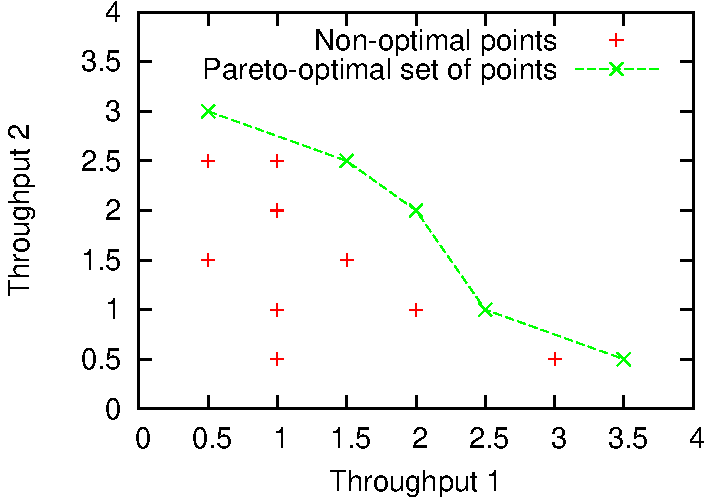
\includegraphics[scale=0.68]{images/pareto}
		\captionof{figure}{Pareto-optimal set in a two-dimensional system}
	   \label{fig:pareto}
	\end{figurehere}

		% subsection state_representation (end)

		\subsection{Comparisons}
		\label{sub:comparisons}
		For this research the algorithm can be compared to the turn-based
		implementation where each agent may only send a message in its own turn.
		% subsection comparisons (end)

		% FIXME: number of states+actions
		% FIXME: Something about how easy it is to extend to multiple channels
	% section approach (end)

	\end{multicols}
	\section{Results}
	\label{sec:results}
	Table \ref{tab:turns} shows that the turn-based approach is more efficient
	as the number of agents and the probability of obtaining a new message
	increases. This is because after the all agents have had their first turn,
	the probability of having a message to send is $P(m)^n$, as there are
	$n$ times that a new message can fill the buffer with probability $P(m)$.

	\begin{table}[h]
		\centering
		\begin{tabular}{|r|rrrrr|}
			\hline
			& 1 agent & 2 agents & 3 agents& 4 agents& 5 agents\\
			\hline
			$p=0.1$ & 100157 & 190211 & 271604 & 344064 & 410397\\
			$p=0.2$ & 200015 & 360030 & 488788 & 590683 & 672028\\
			$p=0.5$ & 500050 & 749407 & 875208 & 937568 & 968696\\
			$p=0.7$ & 699996 & 909630 & 972937 & 991940 & 997638\\
			\hline
		\end{tabular}
		\caption{Total throughput for turn-based policy after 1000000 turns}
		\label{tab:turns}
	\end{table}

	In figure \ref{fig:t2s0} we see that the size of the Pareto front is not
	uniform for all probability distributions. The sizes are smallest where
	probabilities are $0.5$ and on the diagonals of the quadrants. The
	smaller set sizes represent the fact that these probability distributions
	produce more duplicate vectors, which are only included once in the sets.
	\newgeometry{textwidth=\paperwidth,layoutvoffset=.75cm,textheight=\paperheight}
	\begin{figure}
		\centering
		\begin{subfigure}[b]{0.3\textwidth}
			\centering
			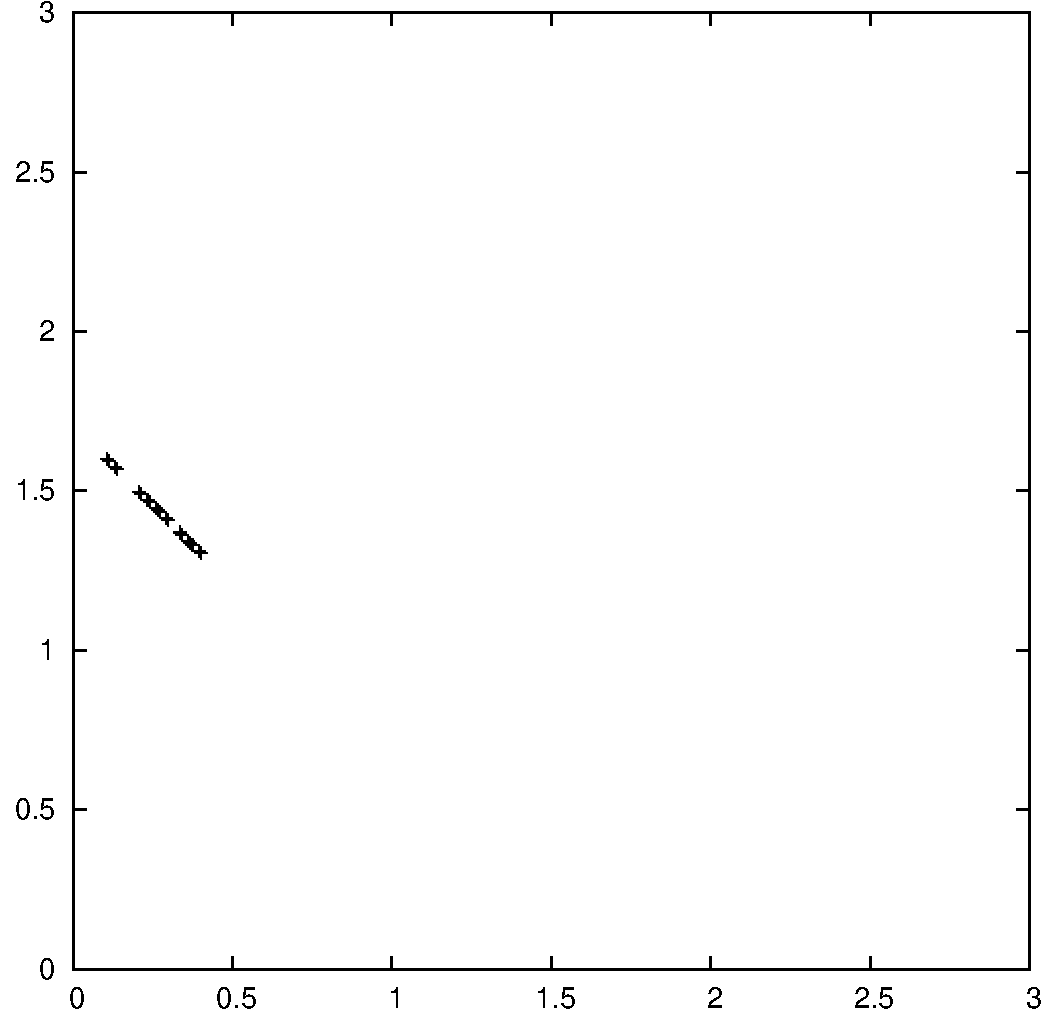
\includegraphics[width=\textwidth]{images/t2s0}
			\caption{s=(e,e)}
			\label{fig:t2s0}
		\end{subfigure}
		~
		\begin{subfigure}[b]{0.3\textwidth}
			\centering
			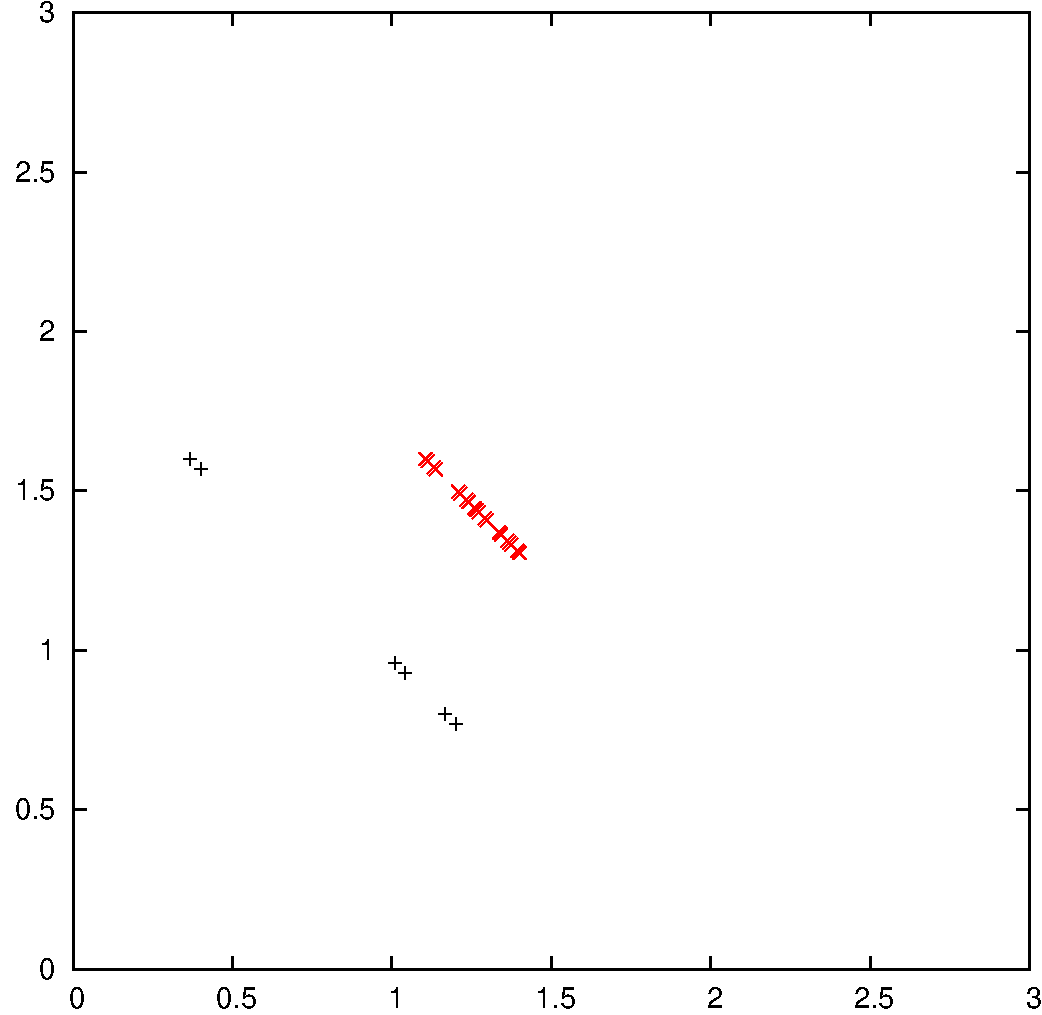
\includegraphics[width=\textwidth]{images/t2s1}
			\caption{s=(m,e)}
			\label{fig:t2s1}
		\end{subfigure}
		~
		\begin{subfigure}[b]{0.3\textwidth}
			\centering
			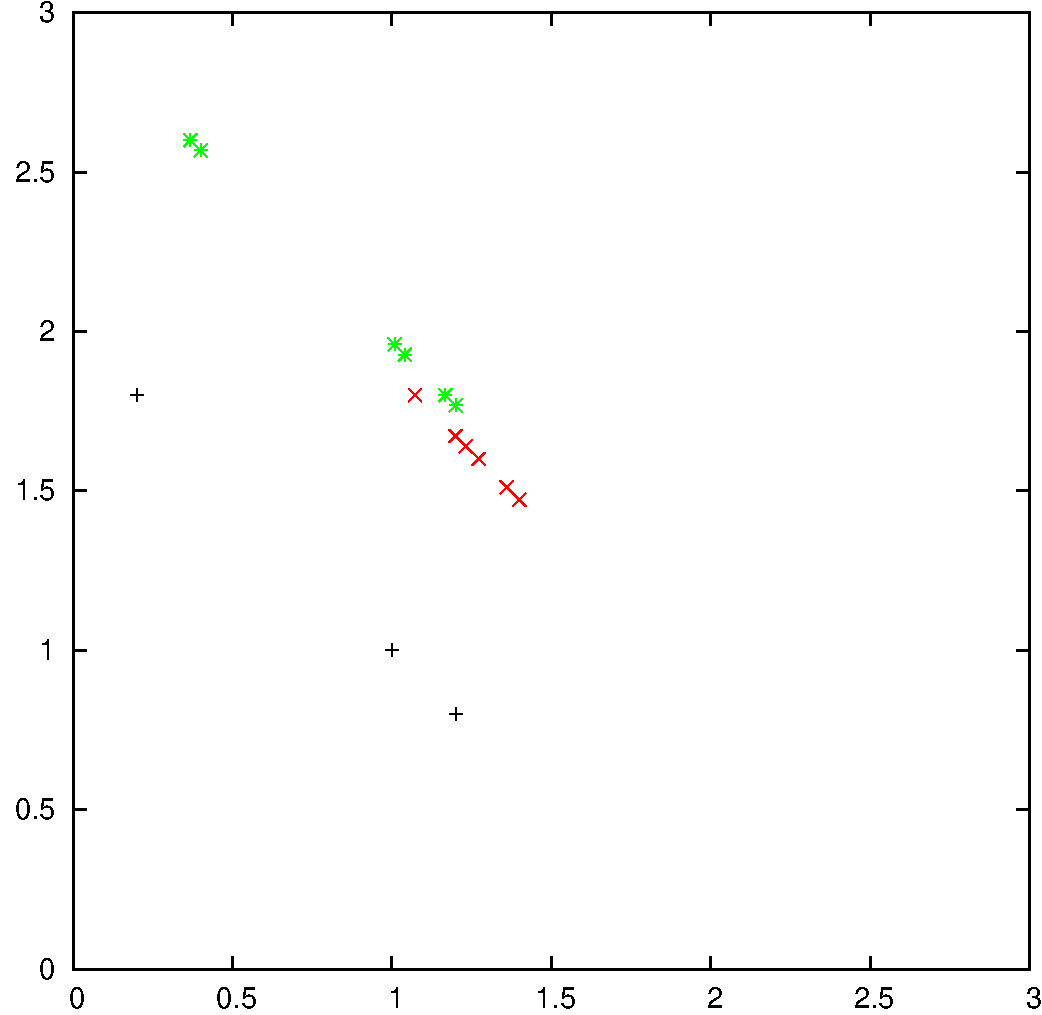
\includegraphics[width=\textwidth]{images/t2s3}
			\caption{s=(m,m)}
			\label{fig:t2s3}
		\end{subfigure}
		\caption{Time step 2}
	\end{figure}

	\begin{figure}
		\centering
		\begin{subfigure}[b]{0.3\textwidth}
			\centering
			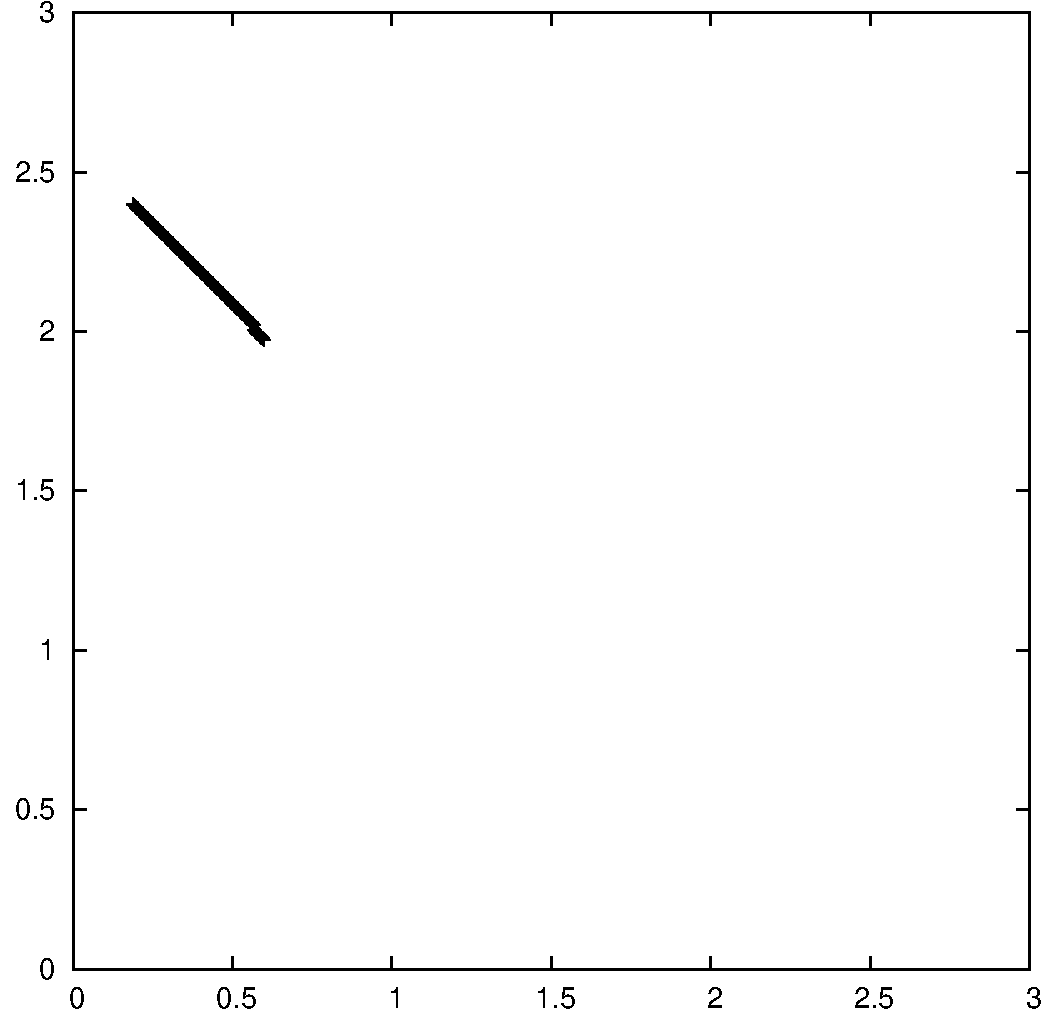
\includegraphics[width=\textwidth]{images/t3s0}
			\caption{s=(e,e)}
			\label{fig:t3s0}
		\end{subfigure}
		~
		\begin{subfigure}[b]{0.3\textwidth}
			\centering
			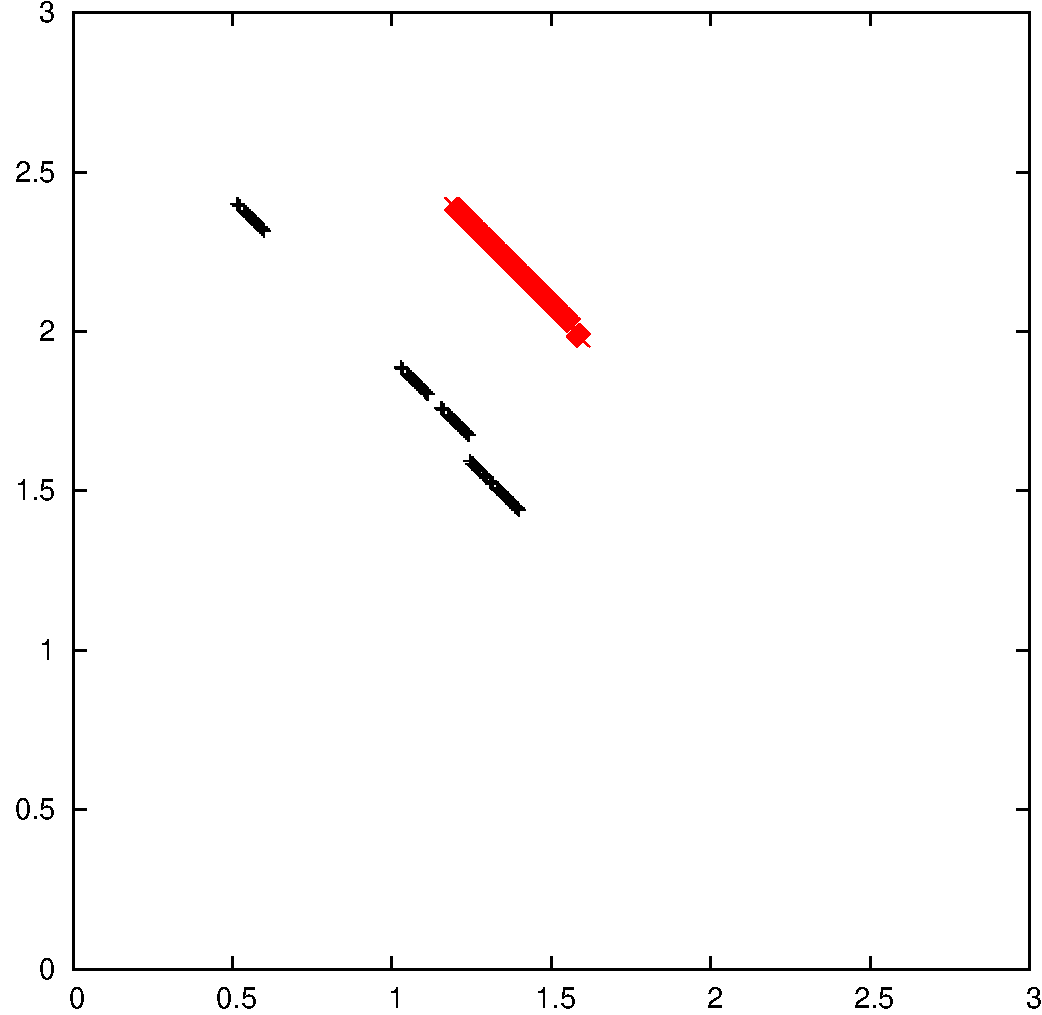
\includegraphics[width=\textwidth]{images/t3s1}
			\caption{s=(m,e)}
			\label{fig:t3s1}
		\end{subfigure}
		~
		\begin{subfigure}[b]{0.3\textwidth}
			\centering
			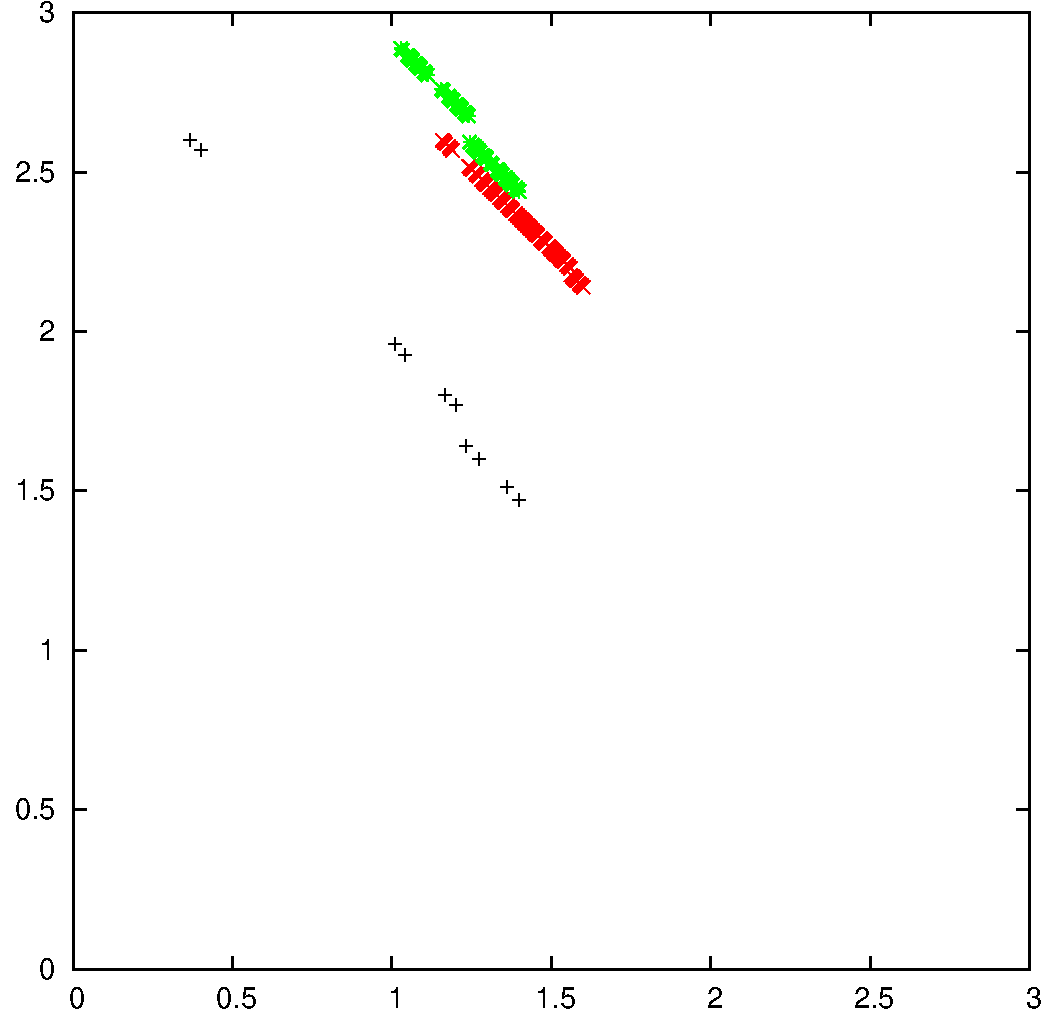
\includegraphics[width=\textwidth]{images/t3s3}
			\caption{s=(m,m)}
			\label{fig:t3s3}
		\end{subfigure}
		\caption{Time step 3}
	\end{figure}

	\begin{figure}
		\centering
		\begin{subfigure}[b]{0.45\textwidth}
			\centering
			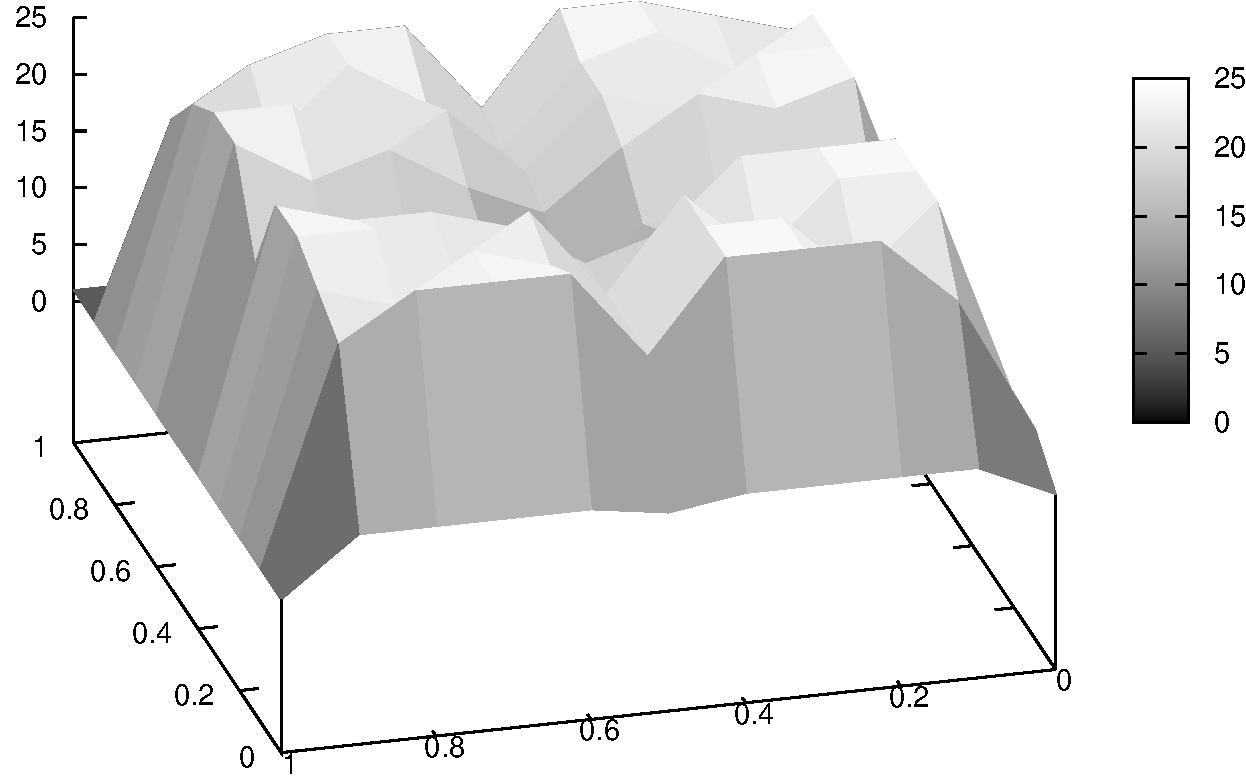
\includegraphics[width=\textwidth]{images/r3_side}
			\caption{From the side}
			\label{fig:r3_side}
		\end{subfigure}
		~
		\begin{subfigure}[b]{0.45\textwidth}
			\centering
			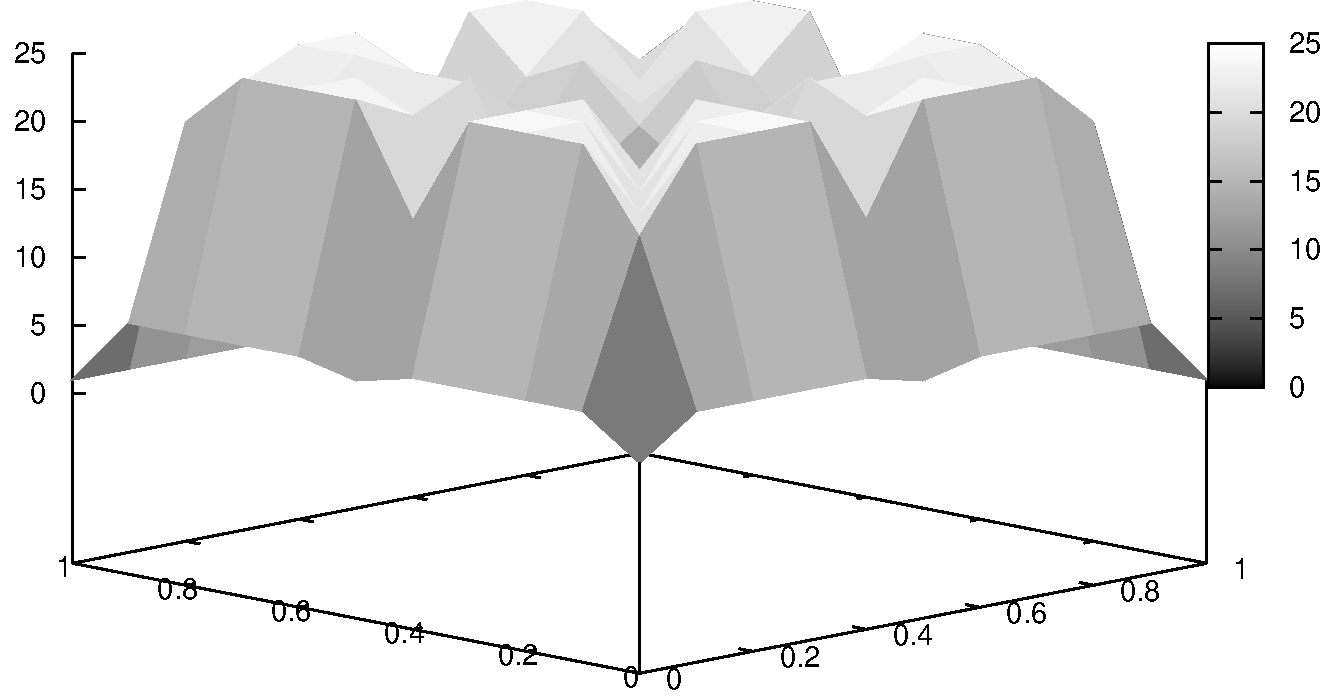
\includegraphics[width=\textwidth]{images/r3_diagonal}
			\caption{Diagonally}
			\label{fig:r3_diagonal}
		\end{subfigure}

		\begin{subfigure}[b]{0.45\textwidth}
			\centering
			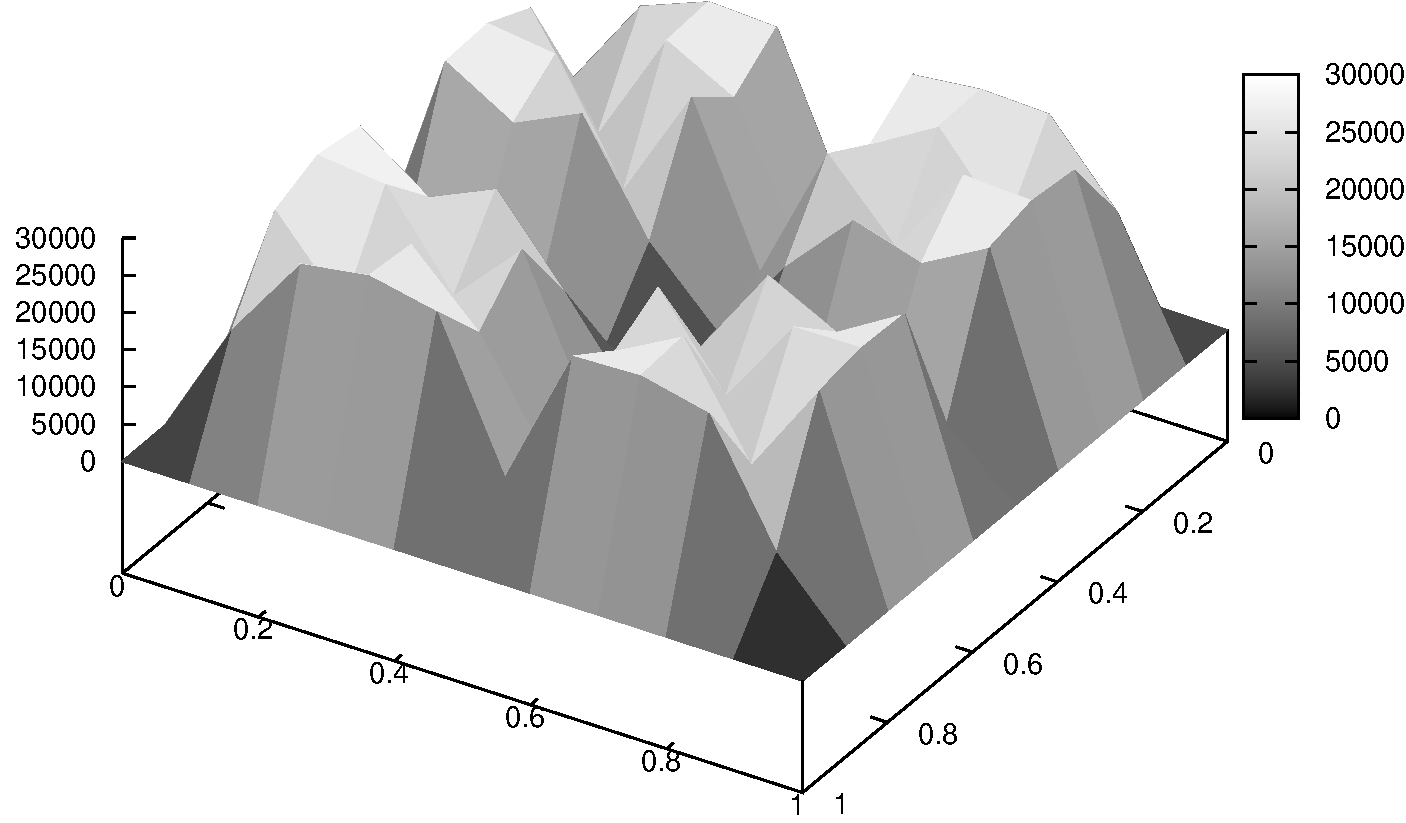
\includegraphics[width=\textwidth]{images/r3_nopareto}
			\caption{Without pareto-optimisation}
			\label{fig:r3_nopareto}
		\end{subfigure}
		~
		\begin{subfigure}[b]{0.45\textwidth}
			\centering
			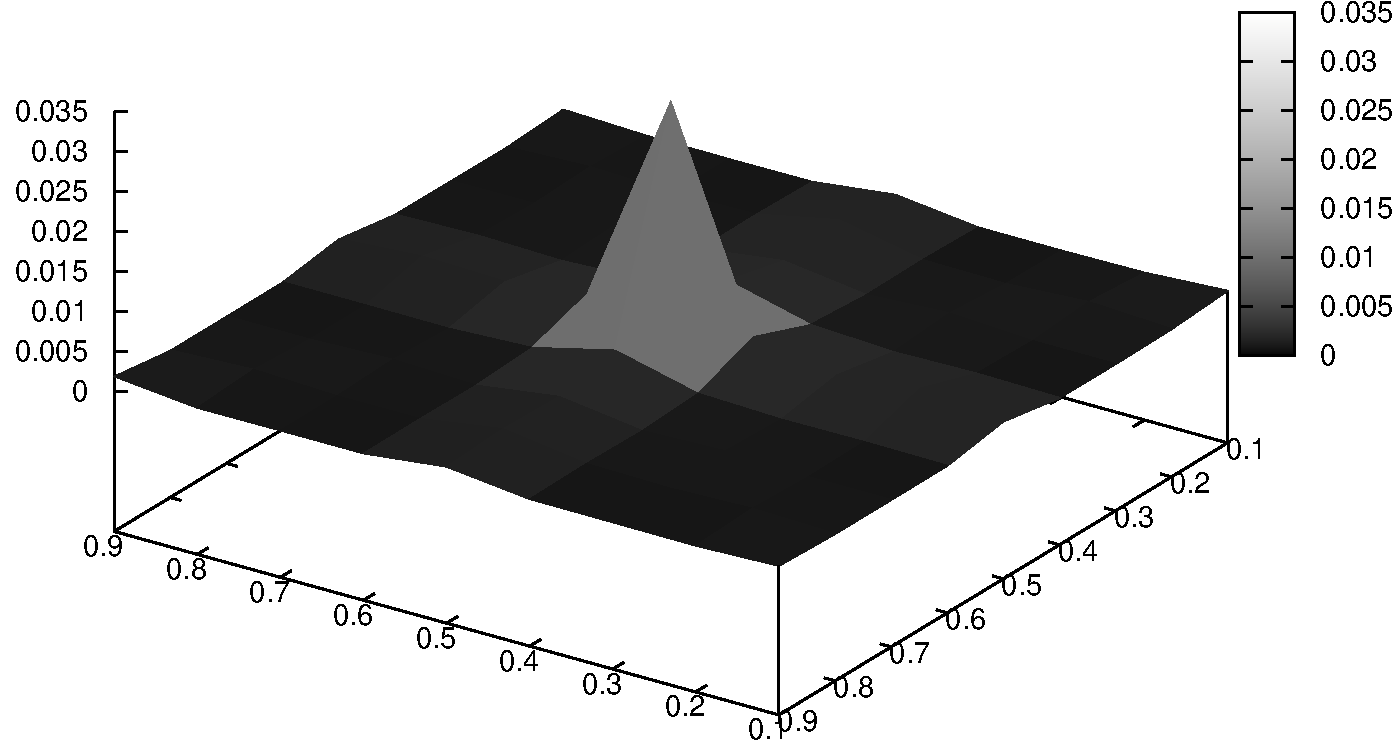
\includegraphics[width=\textwidth]{images/r3_divided}
			\caption{With optimisation / without}
			\label{fig:r3_divided}
		\end{subfigure}
		\caption{Size of the pareto-front over different probability
		distributions, t=3.}
	\end{figure}

	\begin{figure}
		\centering
		\begin{subfigure}[b]{0.45\textwidth}
			\centering
			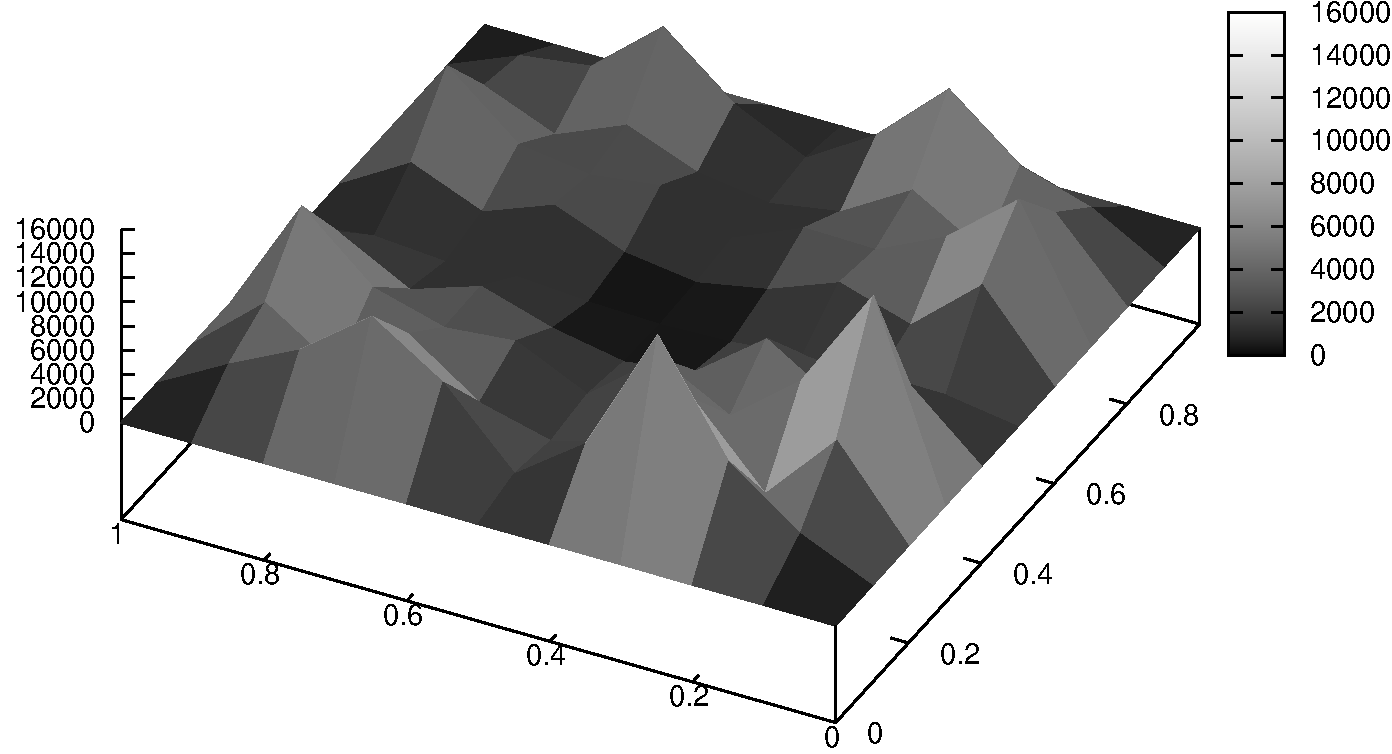
\includegraphics[width=\textwidth]{images/r4_bird}
			\caption{Overview}
			\label{fig:r4_bird}
		\end{subfigure}
		~
		\begin{subfigure}[b]{0.45\textwidth}
			\centering
			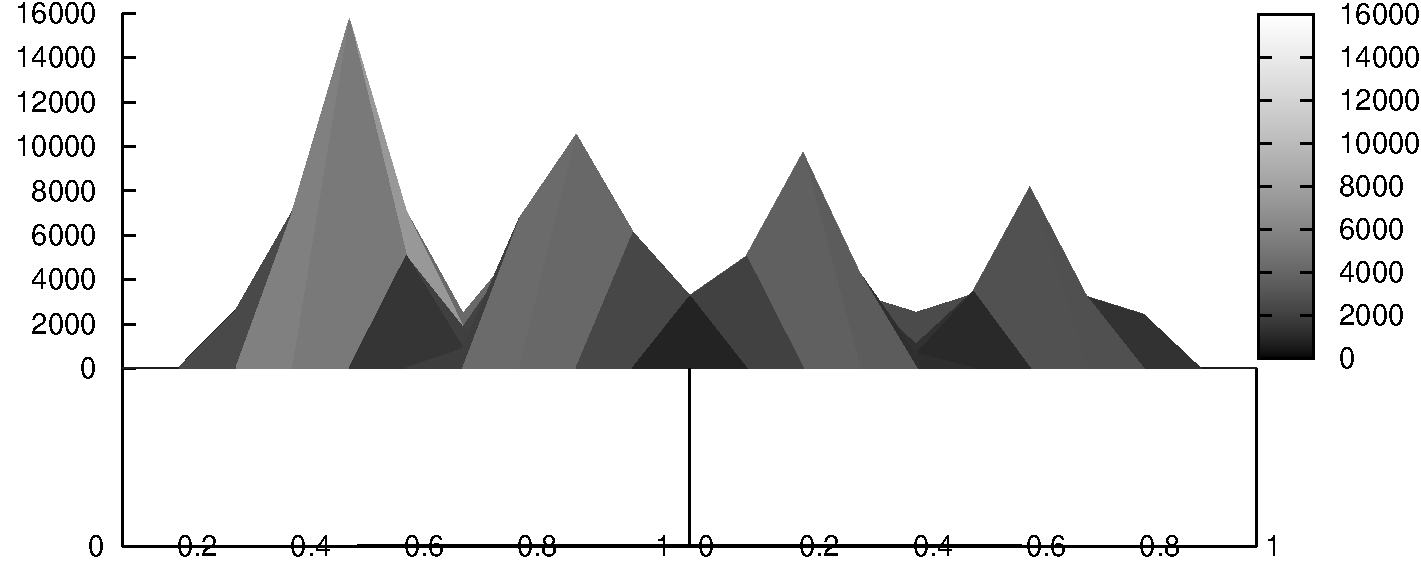
\includegraphics[width=\textwidth]{images/r4_diagonal}
			\caption{Diagonally}
			\label{fig:r4_diagonal}
		\end{subfigure}
		\caption{Size of the pareto-front over different probability
		distributions, t=4.}
	\end{figure}

	\begin{figure}
		\centering
		\begin{subfigure}[b]{0.45\textwidth}
			\centering
			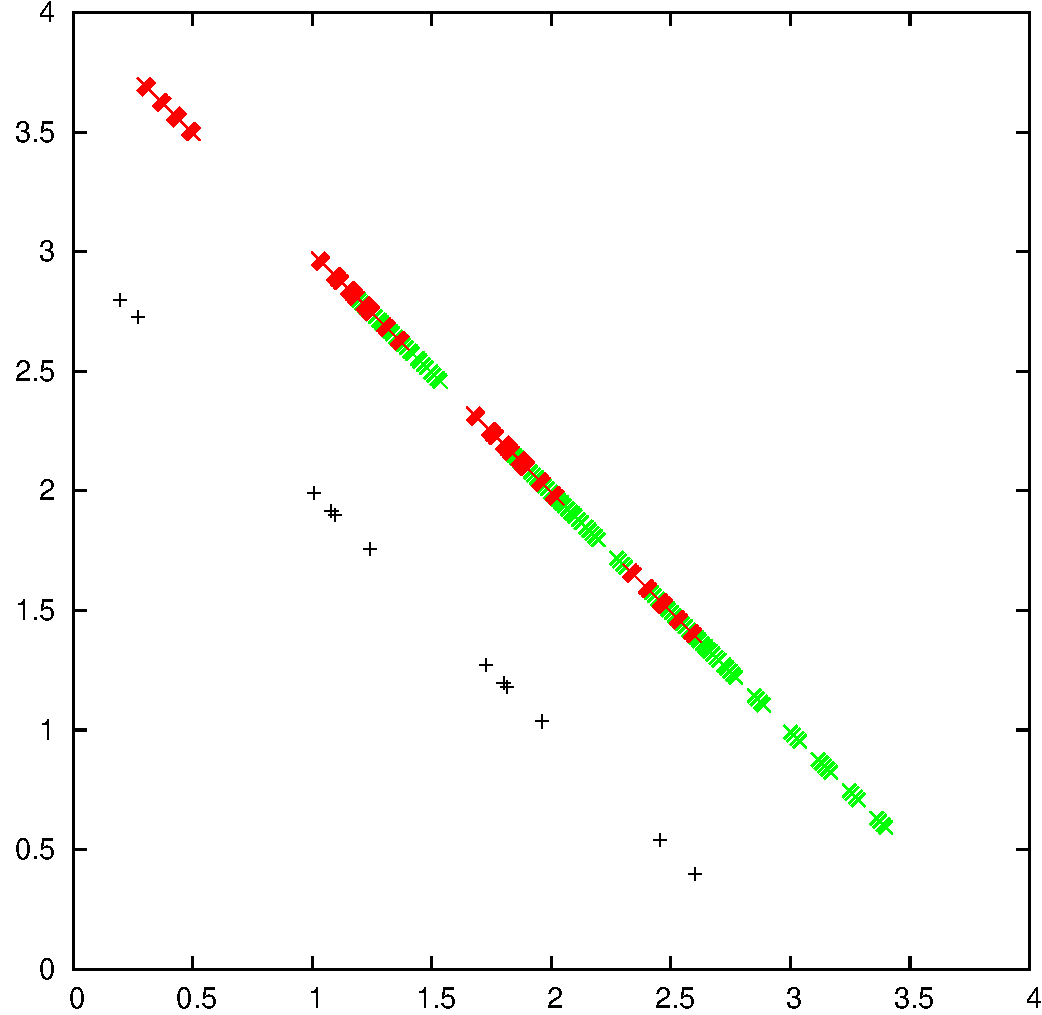
\includegraphics[width=\textwidth,height=7cm,keepaspectratio]{images/t4_12}
			\caption{t=4, p=(0.1, 0.2)}
			\label{fig:t4_12}
		\end{subfigure}
		~
		\begin{subfigure}[b]{0.45\textwidth}
			\centering
			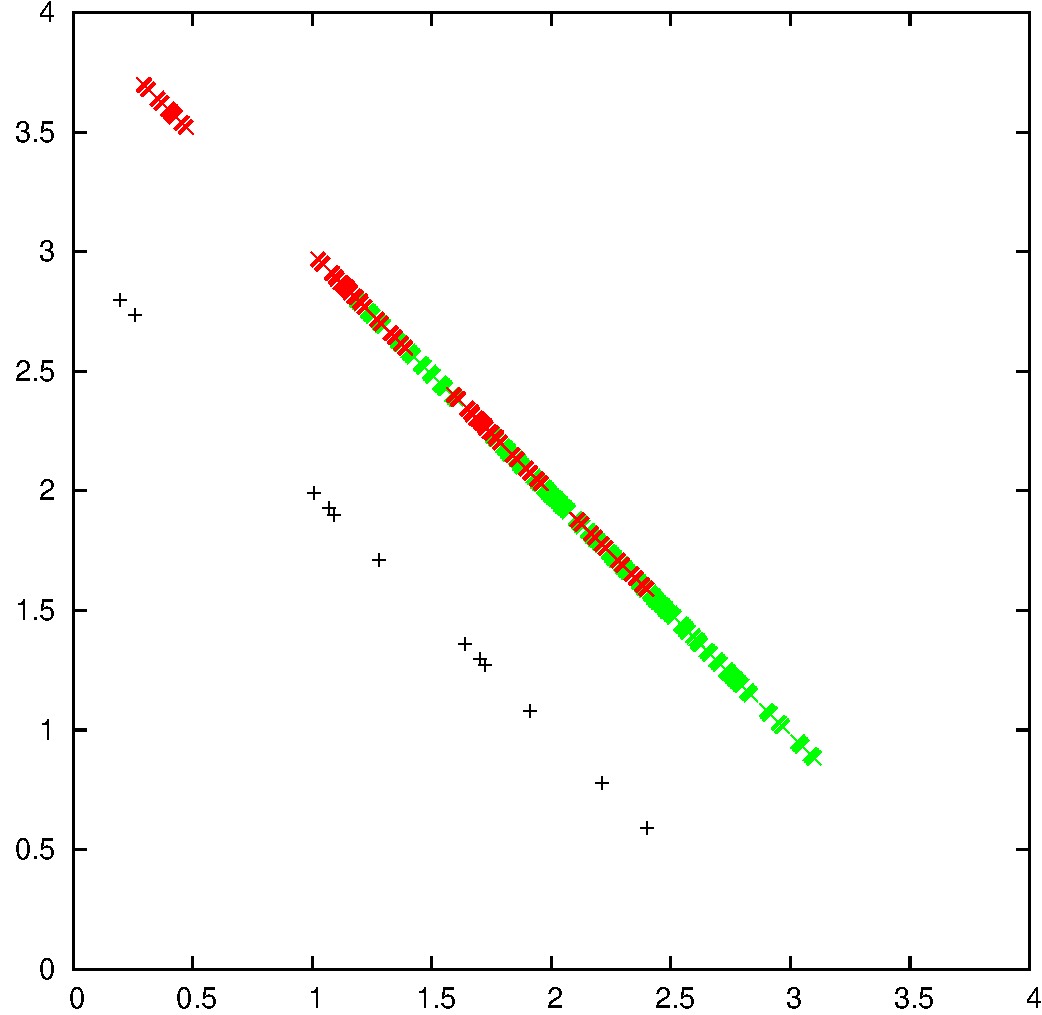
\includegraphics[width=\textwidth,height=7cm,keepaspectratio]{images/t4_13}
			\caption{t=4, p=(0.1, 0.3)}
			\label{fig:t4_13}
		\end{subfigure}

		\begin{subfigure}[b]{0.45\textwidth}
			\centering
			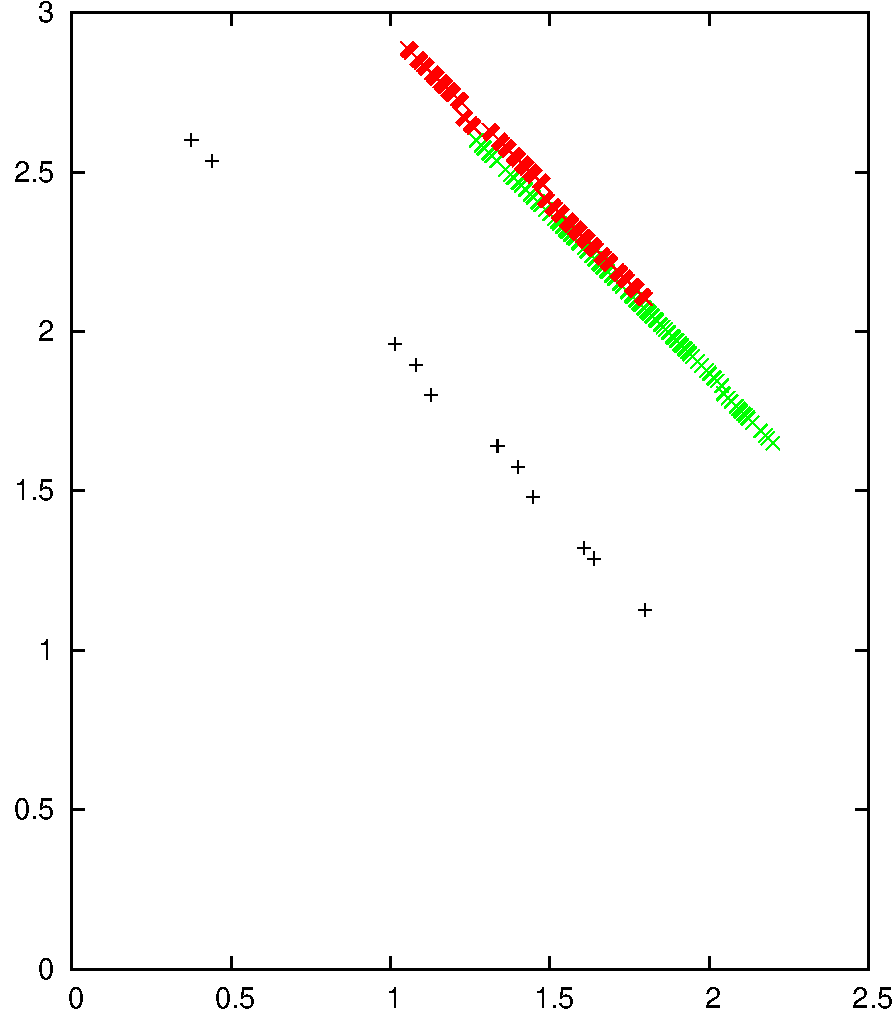
\includegraphics[width=\textwidth,height=7cm,keepaspectratio]{images/t4_26}
			\caption{t=4, p=(0.2, 0.6)}
			\label{fig:t4_26}
		\end{subfigure}
		~
		\begin{subfigure}[b]{0.45\textwidth}
			\centering
			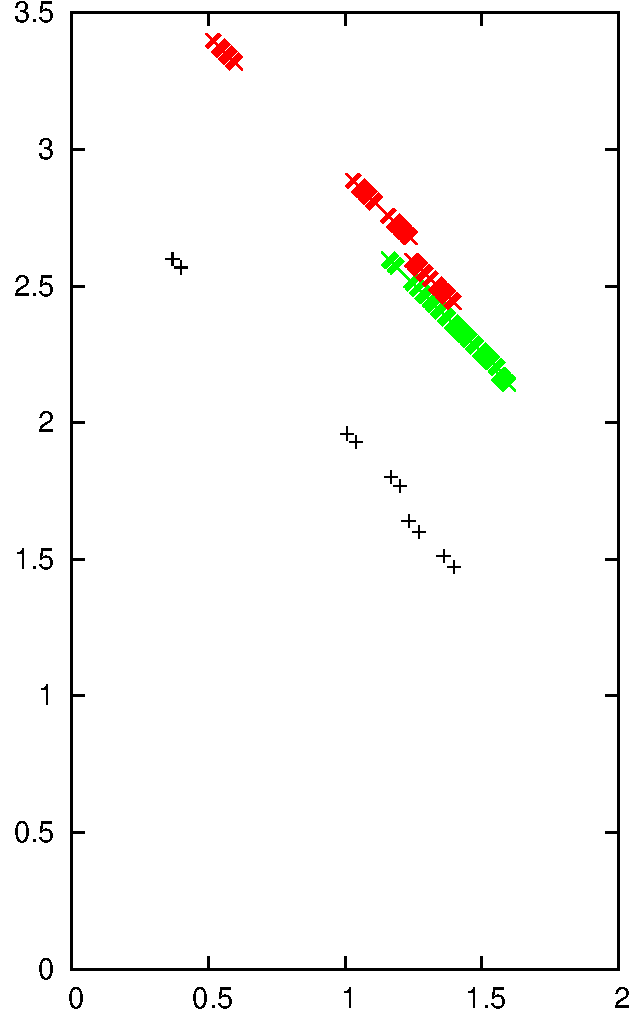
\includegraphics[width=\textwidth,height=7cm,keepaspectratio]{images/t4_28}
			\caption{t=4, p=(0.2, 0.8)}
			\label{fig:t4_28}
		\end{subfigure}

		\begin{subfigure}[b]{0.45\textwidth}
			\centering
			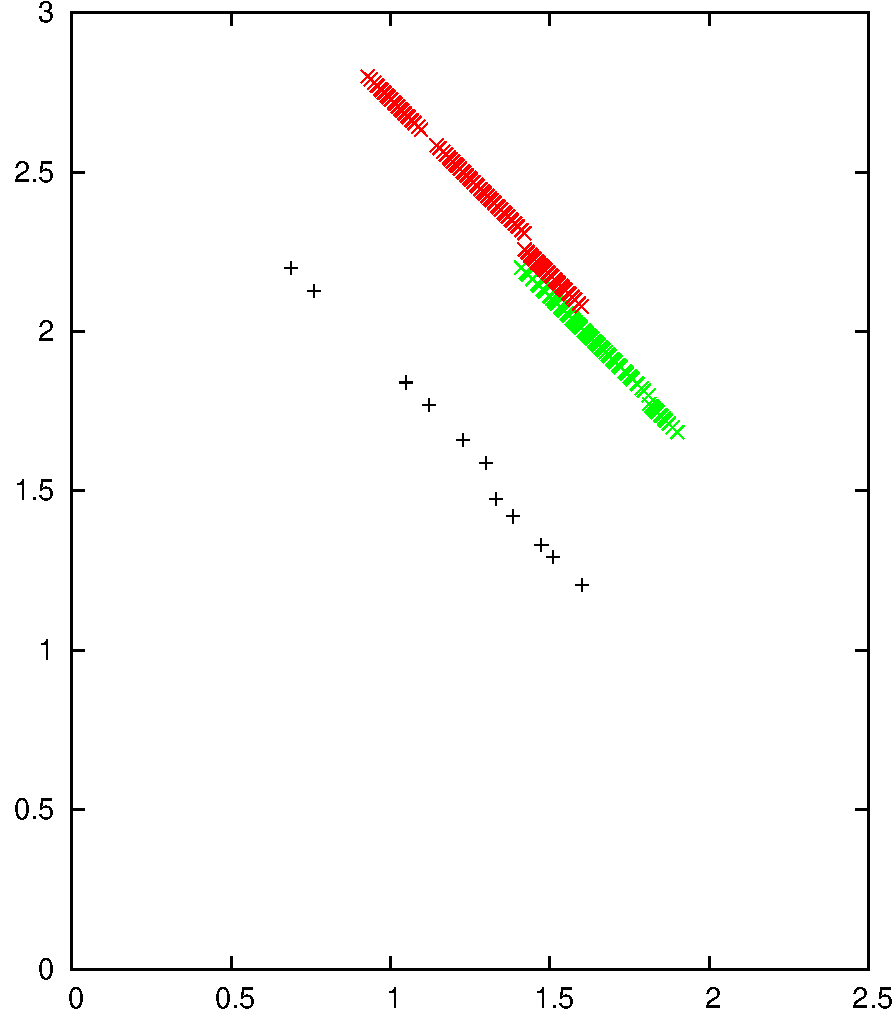
\includegraphics[width=\textwidth,height=7cm,keepaspectratio]{images/t4_47}
			\caption{t=4, p=(0.4, 0.7)}
			\label{fig:t4_47}
		\end{subfigure}
		~
		\begin{subfigure}[b]{0.45\textwidth}
			\centering
			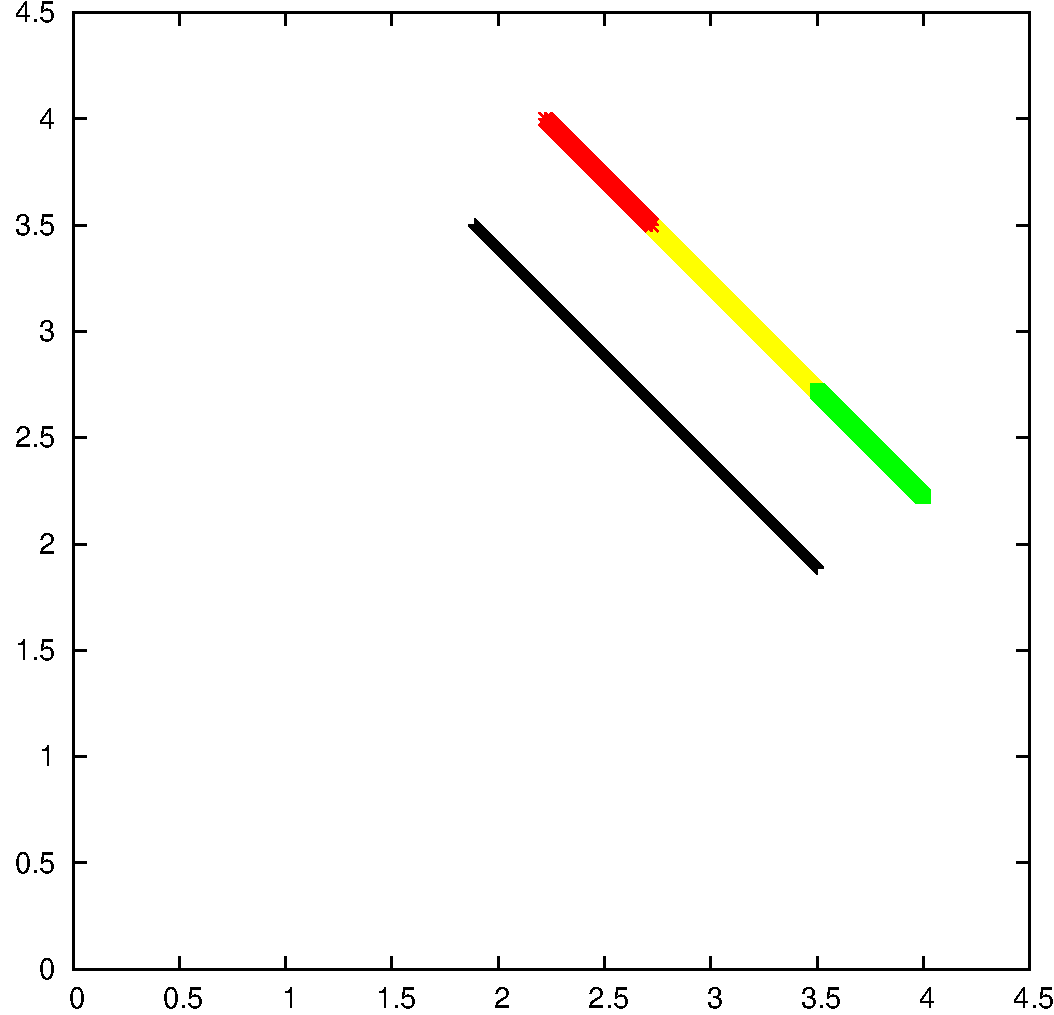
\includegraphics[width=\textwidth,height=7cm,keepaspectratio]{images/t7_55}
			\caption{t=7, p=(0.5, 0.5)}
			\label{fig:t7_55}
		\end{subfigure}
		\caption{Shape of the Pareto-front for different time steps and
		probabilities with two agents}
	\end{figure}

	\begin{figure}
		\centering
		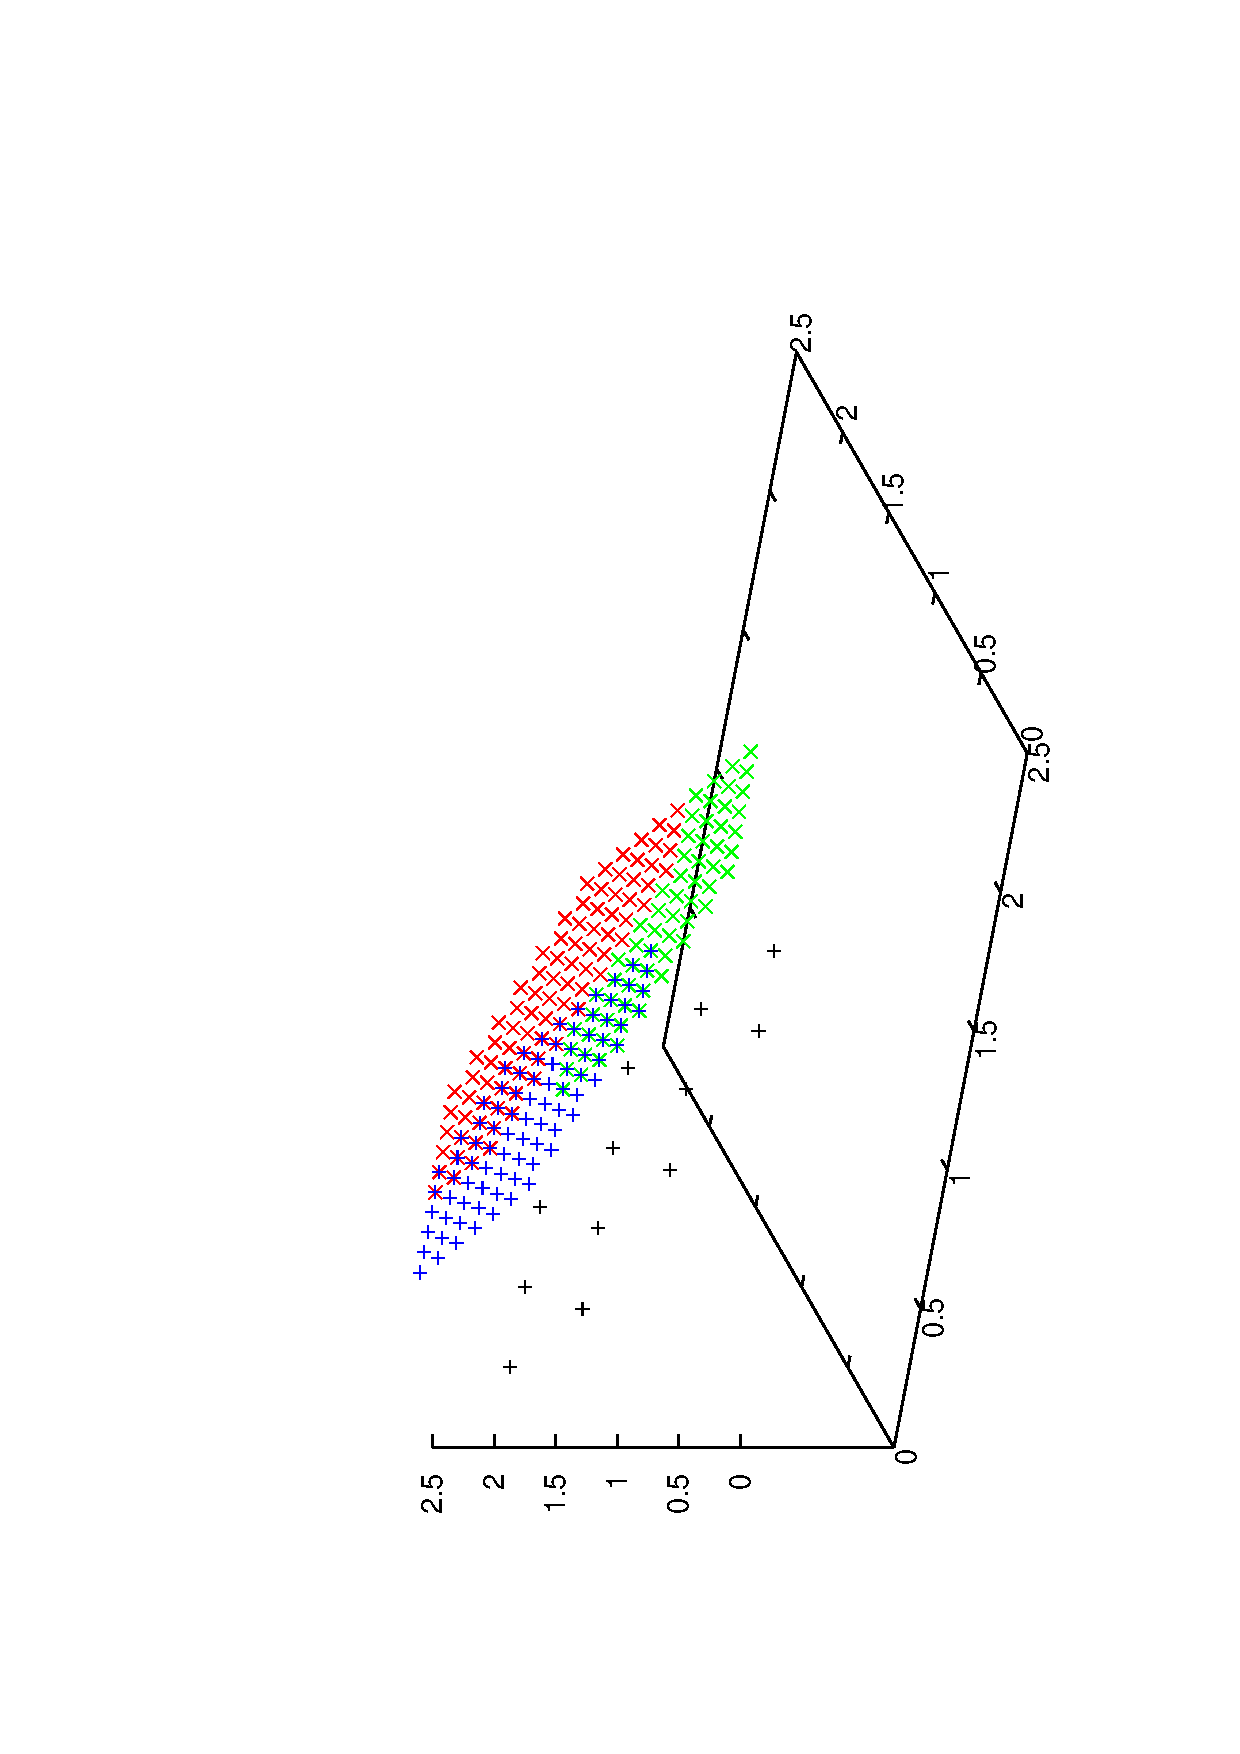
\includegraphics[width=\textwidth,height=10cm,keepaspectratio]{images/t3_555}
		\label{fig:t3_555}
		\caption{t=3, p=(0.5, 0.5, 0.5)}
	\end{figure}

	% FIXME: something about worse than exponential growth
	Figure XXX shows that the size of the Pareto-front grows faster than
	exponentially
	% section results (end)
	\restoregeometry

	\section{Discussion}
	\label{sec:discussion}
	\subsection{Sorted Sets}
	\label{sub:sorted_sets}
	% Reduce time complexity with sorted sets
	As the C++ implementation of the \texttt{set} class is sorted, it is
	possible to select subsets based on separators. In the case of adding a new
	vector to the set there are three distinct possibilities:
	\begin{enumerate}
		\item Elements must be removed and the new vector added
		\item No elements must be removed but the new vector must be added
		\item No elements must be removed and the new vector must not be added
	\end{enumerate}
	When we consider the whole set per dimension, this separates the vectors in
	the set into three different sets of interest:
	\begin{enumerate}
		\item Elements that may be strictly better
		\item Elements that may be strictly worse
		\item Elements that are not better or worse
	\end{enumerate}
	Sets 1 and 2 may intersect when the values of the vector that have been
	compared are the same as the vector that is to be added.

	As the sets are in a large part distributed on a few lines, we could
	represent them as several sets, grouped by the lines they are on. As all
	points are on a single line, the vectors in the set are sorted in both the
	first and the second dimension.

	All points of interest for ruling out that the vector are in the quadrant
	that contains only vectors that are higher or equal to the new vectors in
	the first two dimensions. By using these features we can reduce the amount
	of vectors that need to be compared to about a quarter.
	% FIXME: Explain this better!
	% FIXME: Only works on last two dimensions, only one dimension at the time
	%
	% 1	.9		.4
	% 1	.8		.5
	% 1	.7		.6
	% 1	.6		.7
	% 1	.5		.8
	% 1	.4		.9
	%					<- last two dimensions are sorted; can be categorised in one
	%						go when the first n-2 values are the same
	% 1.1	.8		.5
	% 1.1	.7		.6
	% 1.1	.6		.7
	% 1.1	.5		.8
	% may work if we save all vectors together that start with the same values

	% Should be a tree for the first n-2 dimensions. C++: multimap
	%
	% 0.0	-> 0.0 -> [...]
	%		-> 0.5 -> [...]
	%		-> 1.0 -> [...]
	%		-> 1.5 -> [...]
	%
	% 0.5	-> 0.0 -> [...]
	%		-> 0.5 -> [...]
	%		-> 1.0 -> [...]
	%		-> 1.5 -> [...]
	%
	% 1.0	-> 0.0 -> [...]
	%		-> 0.5 -> [...]
	%		-> 1.0 -> [...]
	%
	% 1.5	-> 0.0 -> [...]
	%		-> 0.5 -> [...]
	%
	% (n-2 * for (1/2 n))
	% (1/2)^(n-2)*2*log(n)

	% discovering in which line(/hyperplane) a vector is (for adding):
	% unique key of hyperplane: norm of orthogonal projection on [1 1 1 1 1 ...]
	% = abs(dot(v, n/|n|)) met n = [1 1 1 1]'/norm (with error margin)

	% subsection sorted_sets (end)

	\subsection{Aggressive Pruning}
	\label{sub:aggressive_pruning}
	% Reduce size by cutting on set size
	% subsection aggressive_pruning (end)
	% section discussion (end)
	\pagebreak

	\bibliographystyle{plainnat}
	\bibliography{references}
\end{document}

